\section[Comparação com outras tecnologias para jogos
casuais]{COMPARAÇÃO COM OUTRAS TECNOLOGIAS PARA JOGOS CASUAIS}

Com base nas funcionalidades apresentadas sobre as tecnologias que
fazem parte da especificação do HTML5, será feita uma comparação com
as principais ferramentas utilizadas para o desenvolvimento de jogos
na data da escrita desse trabalho. Para fim de avaliação serão
utilizados os quesitos performance, portabilidade, fragmentação e recursos para
desenvolvimento.

\subsection{Outras tecnologias utilizadas atualmente}

Com exceção do HTML5, as ferramentas atuais para desenvolvimento de jogos para a internet se
utilizam de extensões que são instaladas nativamente no computador,
essas extensões interpretam o código gerado pelo desenvolvedor e
executam o mesmo nativamente no dispositivo para obter um melhor
acesso ao hardware. A utilização de extensões de terceiros para a
executação de um jogo possui várias vantagens e desvantagens, e esse
capítulo visa mostrar quais são e compará-las com o que o HTML provê.
Essas tecnologias mais utilizadas para desenvolvimento de jogos são
Java, Flash e Unity3D.

\subsubsection{Java}

Java foi uma das primeiras tecnologias portada para os navegadores que podia proporcionar um
ambiente favorável ao desenvolvimento de games. Para que essa funcionalidade ficasse disponível para os
navegadores, a plataforma Java disponibilizou um segundo tipo de
aplicação chamado \textit{applet}.

Os applets são programas Java que podem ser inseridos em uma página de
internet. \cite{boese2009introduction}. Esses programas são inseridos nas
páginas utilizando a tag \textit{<applet>} no documento HTML passando
o arquivo Java em um dos seus atributos. Com isso o programa Java é
baixado do servidor e executado na maquina do cliente pelo navegador,
que utiliza um ambiente de \textit{sandbox}, assim não permitindo
ao programa ter total acesso dentro da maquina do usuário.

Durante um bom período de tempo a plataforma Java foi a única tecnologia
aceitável para se colocar um jogo disponível via internet, até que
novas tecnologias começaram a surgir e a plataforma Java perdeu um pouco do seu
espaço como tecnologia para desenvolvimento de jogos para internet,
apesar dele ainda ser utilizado por alguns, principalmente no meio
acadêmico.

\subsubsection{Flash}

Flash é um produto criado pela Macromedia em 1996, com a finalidade de
enriquecer o conteúdo da internet, trazendo funcionalidades que não
era possível disponibilizar apenas com HTML na época de sua criação.
Com Flash, foi possível a criação de diversos sites com animações, e
foi o que originou as home pages animadas com um "Clique para entrar".

Em 2005 a Macromedia foi comprada pela Adobe e vem sendo mantido por
ela desde então, juntamente com todo o pacote de multimidia da
Macromedia.

A facilidade em gerar animações com o Flash trouxe a idéia de
utilizá-lo para a criação de jogos que funcionassem diretamente no
navegador, tendo em vista que \textit{plugin} do Flash exporta um binário para ser
executado utilizando o Flash player instalado pelo usuário, a
performance pode ser bem melhor, pois o flash player tem acesso ao
hardware do dispositivo no qual ele está instalado.

Atualmente, Flash é a tecnologia mais utilizada para desenvolvimento de jogos para a
internet. \cite{website:adobeflashleading}. Essa ferramenta possui muitas
bibliotecas feitas para facilitar o desenvolvimento de jogos, e por
possuir uma interface simples tanto para o designer como para o desenvolvedor,
ela vem mantendo seu legado ao longo dos anos.
Mais de 99 por cento dos computadores pessoais possuem o Flash Player
instalado. \cite{website:adobeflashpenetration}. E esse é um dos grandes
motivos do sucesso do Flash, pois quebra um dos grandes problemas de
se desenvolver um jogo que necessita de dependencias externas para ser
executado.

\subsubsection{Unity3D}

Conforme \citeonline{blackman2011beginning}, a \textit{engine} Unity3D provê
um bom ponto de entrada para o mundo do desenvolvimento de jogos, pois
ela possui um bom balanceamento entre funcionalidades e um bom preço.

Unity3D é uma \textit{engine} relativamente nova para desenvolvimento de jogos e está
ganhando muito espaço no mercado devido a sua facilidade de uso e
aumento na popularidade dos seus \textit{plugins}. Utilizando-a é possível
desenvolver apenas um jogo e exportá-lo para ser executado em
diferentes plataformas, entre elas o navegador, que utiliza um
\textit{plugin} para executá-lo, e a quantidade de instalações do \textit{plugin} já
ultrapassa 35 milhões. \cite{blackman2011beginning}.

A \textit{engine} Unity3D é o principal produto da empresa
Unity. \cite{website:unity3dcompany}. Esse produto é uma \textit{engine}
que possui como foco facilitar o desenvolvimento de jogos no
geral, tirando do desenvolvedor a preocupação de criar um jogo para
diversas plataformas, assim deixando-o mais livre para pensar nas
funcionalidades do seu próprio jogo e também prover um ambiente
simples para esse desenvolvimento, dando-lhe ferramentas gráficas que
facilitam a criação dos personagens e mapas do jogo, tanto para jogos
3D, que são o foco principal da \textit{engine}, como para jogos 2D
que podem se utilizar do 3D para a criação de um jogo que faça uma
simulação simples de 2D,

É possível exportar jogos para rodar diretamente no navegador, mas
esse não é o único caminho que a \textit{engine} Unity3D fornece, é possível exportar
para Windows, Mac e outros dispositivos que já possuem versões do
Unity3D rodando.

Apesar de possuir uma versão paga com muitas vantagens e novas
funcionalidades muito úteis para empresas de jogos, essa engine possui
também uma versão gratuita que permite ao desenvolvedor criar,
aprender e até mesmo vender os seus jogos sem precisar pagar nada, e
isso tem sido um dos grandes atrativos de novos desenvolvedores.

Essa engine vem crescendo bastante desde seu lançamento em 2009 e vem ganhando
cada vez mais novas pessoas na comunidade, que já possui mais de
400.000 (em abril de 2011 conforme
\citeonline{blackman2011beginning}), e vem disputando a fama de melhor plataforma
para desenvolvimento de jogos para o navegador.

O site oficial do Unity3D possui alguns jogos que foram feitos para
navegador, detalhes podem ser vistos em \citeonline{website:unity3dwebgames}.
Para que os jogos sejam executados o jogador precisa
necessariamente instalar o Unity web player para que o jogo seja executado.
Tal player está disponível para download no site da empresa. \cite{website:unity3dwebplayer}.

\subsection{Performance}
%usar isso http://www.timo-ernst.net/2010/09/a-scientific-performance-comparison-flexflash-vs-javafx-vs-silverlight-vs-javascript/
%http://www.mikechambers.com/blog/2010/03/01/relative-performance-of-rich-media-content-across-browsers-and-operating-systems/
%http://www.readwriteweb.com/archives/does_html5_really_beat_flash_surprising_results_of_new_tests.php

Performance é um assunto muito discutido no desenvolvimento de jogos
pois eles consomem muito processamento, memória e IO do dispositivo em que estão
executando, pois estão, entre outras coisas, em constante execução, fazendo
cálculos diversos para situar o jogador dentro do jogo por exemplo.
Entre esses cálculos, dependendo do jogo, estão os cálculos de física dos
objetos da cena e do próprio jogador, transformação de imagens para
dar impressão de movimento ou sombra e outras coisas que exigem alto
processamento em um curto período de tempo.

As tecnologias que exigem a instalação de um software de terceiros
(Java, Unity3D e Flash) tendem a possuir uma performance melhor em alguns casos
e pior em outros no momento de escrita desse trabalho. De acordo com \citeonline{performanceria},
o navegador teoricamente não deveria influenciar a performance de uma aplicação
feita utilizando uma tecnologia que exige um \textit{plugin} externo, mas isso acontece
em alguns casos, fazendo com que a aplicação perca um pouco em performance.

Um dos possíveis motivos do ganho de performance das tecnologias que
utilizam \textit{plugins} externos é a otimização da plataforma para utilização em um determinado
dispositivo, assim ganhando várias vantagens como um processo separado no
sistema, apenas executando um jogo que foi previamente "compilado"
especialmente para essa tecnologia.

O HTML5 juntamente com Javascript perde um pouco em performance, pois
o sistema operacional vê apenas um navegador como processo, e esse
navegador vai fazer a interface entre o jogo e o sistema operacional.
O navegador não é uma plataforma otimizada para jogos (como é o caso
de alguns \textit{plugins}, que possuem apenas essa finalidade, ou são bem
direcionados para o tal), apesar de estar em constante evolução e
desenvolvimento para interpretar Javascript de uma maneira mais veloz,
a cada nova versão.

Baseando-se nos testes de \citeonline{performanceria}, é possível notar que
cada tecnologia possui pontos fortes e fracos em termos de performance, sendo que
em muitos casos o Javascript consegue vantagem sobre as outras tecnologias.

\begin{figure}[H]
  \centering
	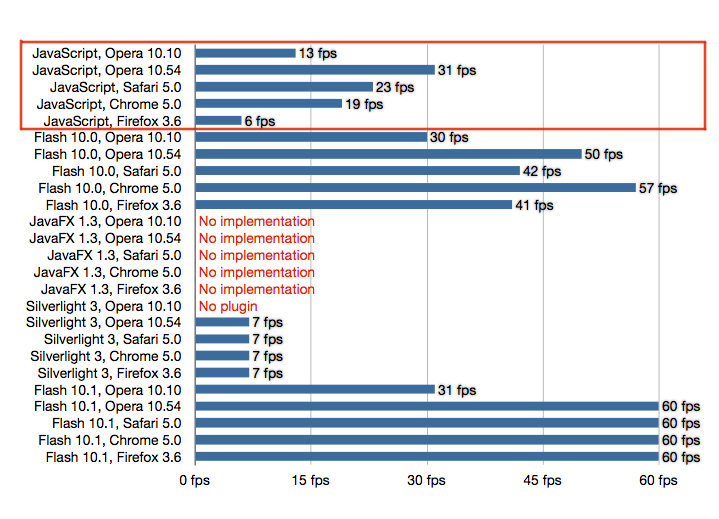
\includegraphics[height=\imgheight,width=\imgwidth]{chart-performance-timo}
	\footnotesize\hspace{8\baselineskip}
	Gráfico 1: Teste de performance 2D \\
	Fonte: \cite{performanceria}
  \label{img:chart-performance-timo}
\end{figure}

No Gráfico 1 criado por \citeonline{performanceria} é
possível ver a diferença de performance entre diferentes tecnologias para a
renderização de gráficos 2D.
Levando em consideração a tecnologia que possui melhor performance,
ou seja o Adobe Flash, podemos ver que o HTML5 ainda perde bastante em performance,
mas isso vem melhorando com o desenvolvimento dos navegadores e a melhoria nas
\textit{engines} de Javascript implementadas por eles.

Tendo em vista que o Adobe Flash é o único que possui a quantidade de FPS
(\textit{frames} por segundo) padrão para o desenvolvimento de jogos,
ele será utilizado como comparação com o HTML5.

O teste foi executado neste trabalho para mostrar o quanto a performance do Javascript evoluiu nesse curto
período de tempo desde o desenvolvimento da pesquisa feita por
\citeonline{performanceria}. O teste foi feito utilizando um
computador Macbook Pro, Processador i7, 4GB de memória RAM utilizando o sistema
operacional Mac OSX Lion, executando diversos navegadores.

\begin{figure}[H]
  \centering
	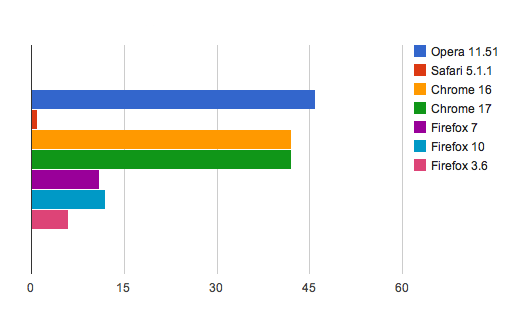
\includegraphics[height=\imgheight,width=\imgwidth]{chart-performance-pothix}
	\footnotesize\hspace{8\baselineskip}
	Gráfico 2: Teste que mostra a performance de um exemplo 2D em Javascript executado na data de escrita desse trabalho
  \label{img:chart-performance-pothix}
\end{figure}

É possível notar no Gráfico 2 que o
Javascript evoluiu mais de 50\% no melhor caso
em relação ao Gráfico 1 e se seguir no mesmo ritmo de evolução
em breve chegará no mesmo patamar do Adobe Flash e será possível obter performances cada
vez melhores mesmo sem utilizar aceleração de hardware.

\begin{figure}[H]
  \centering
	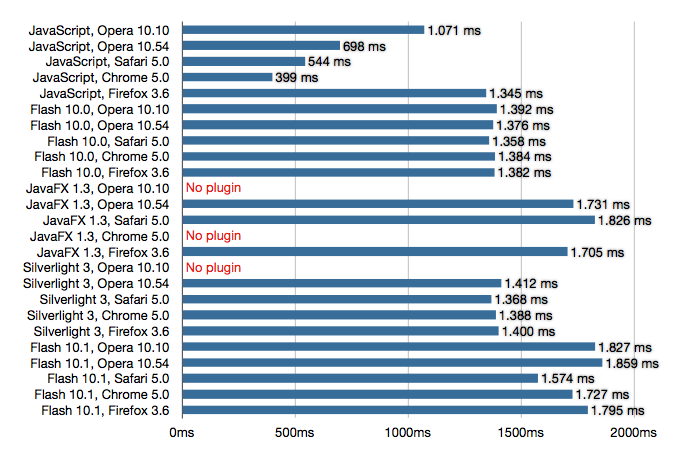
\includegraphics[height=\imgheight,width=\imgwidth]{timo-runlength-benchmark-macos}
	\footnotesize\hspace{8\baselineskip}
	Gráfico 3: Teste de performance para redução de tamanho de string \\
	Fonte: \cite{performanceria}
  \label{img:timo-runlength-benchmark-macos}
\end{figure}

Ainda utilizando os testes feitos por \citeonline{performanceria},
pode-se notar no Gráfico 3 um
caso em que o Javascript consegue vantagem sobre as tecnologias
concorrentes. O teste executado se refere a redução de tamanho de um
determinado texto.

Alem de 2D também é possível utilizar aceleração de hardware para conseguir um quantidade
de \textit{frames} por segundo competitiva entre o Adobe Flash e o
Javascript em algumas plataformas. Para o caso do Javascript é necessário o uso do WebGL para
utilizar essa aceleração. De acordo com os testes feitos por
\citeonline{website:webglvsstage3d}, os valores são bem parecidos entre várias
plataformas, novamente dependendo do suporte do hardware para a
utilização da aceleração.

Os testes criados por \citeonline{website:webglvsstage3d} foram executados
neste trabalho utilizando um Macbook Pro, Processador i7, 4GB de memória RAM com o sistema operacional
Mac OSX Lion e os resultados obtidos podem ser vistos nas Figuras 10
e 11.

\begin{figure}[H]
  \centering
	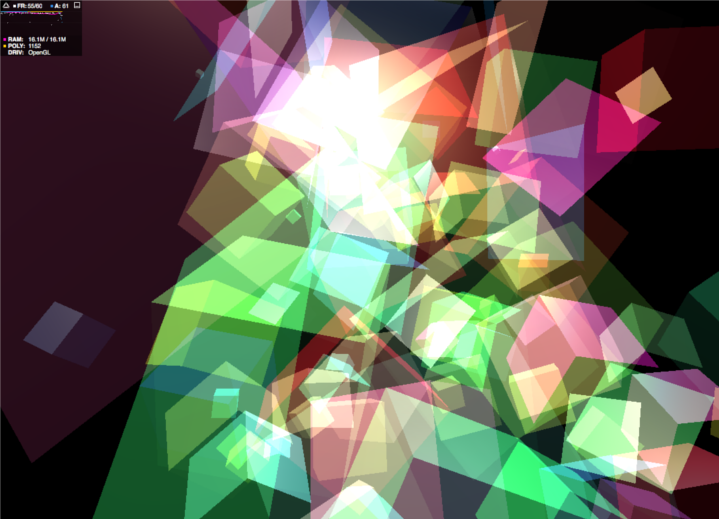
\includegraphics[height=\imgheight,width=\imgwidth]{stage3d-flash-60fps}
	\footnotesize\hspace{8\baselineskip}
	Figura 10: Demo com mais de 100 cubos semi-transparentes sendo
	executado a 60 fps \\
	Fonte: \cite{website:stage3dperformance}
  \label{img:stage3d-flash-60fps}
\end{figure}

A Figura 10 acima mostra a execução da
versão Adobe Flash do experimento, sendo executado entre 55 e 60 fps.
No caso do hardware que é utilizado, o Flash está utilizando OpenGL
para a renderização e consegue uma boa taxa de \textit{frames} por
segundo.

Já a Figura 11 abaixo mostra a execução da
versão WebGL do experimento, também sendo executado a 60 fps no mesmo
hardware. Há bastante divergencia nos testes pois cada pessoa que
executa o teste possui um hardware diferente e pode chegar a
resultados diferentes dependendo do tipo de suporte que o hardware
possui, mas o teste executado para este trabalho mostra que em alguns
hardwares a execução é bem parecida para as duas tecnologias.

\begin{figure}[H]
  \centering
	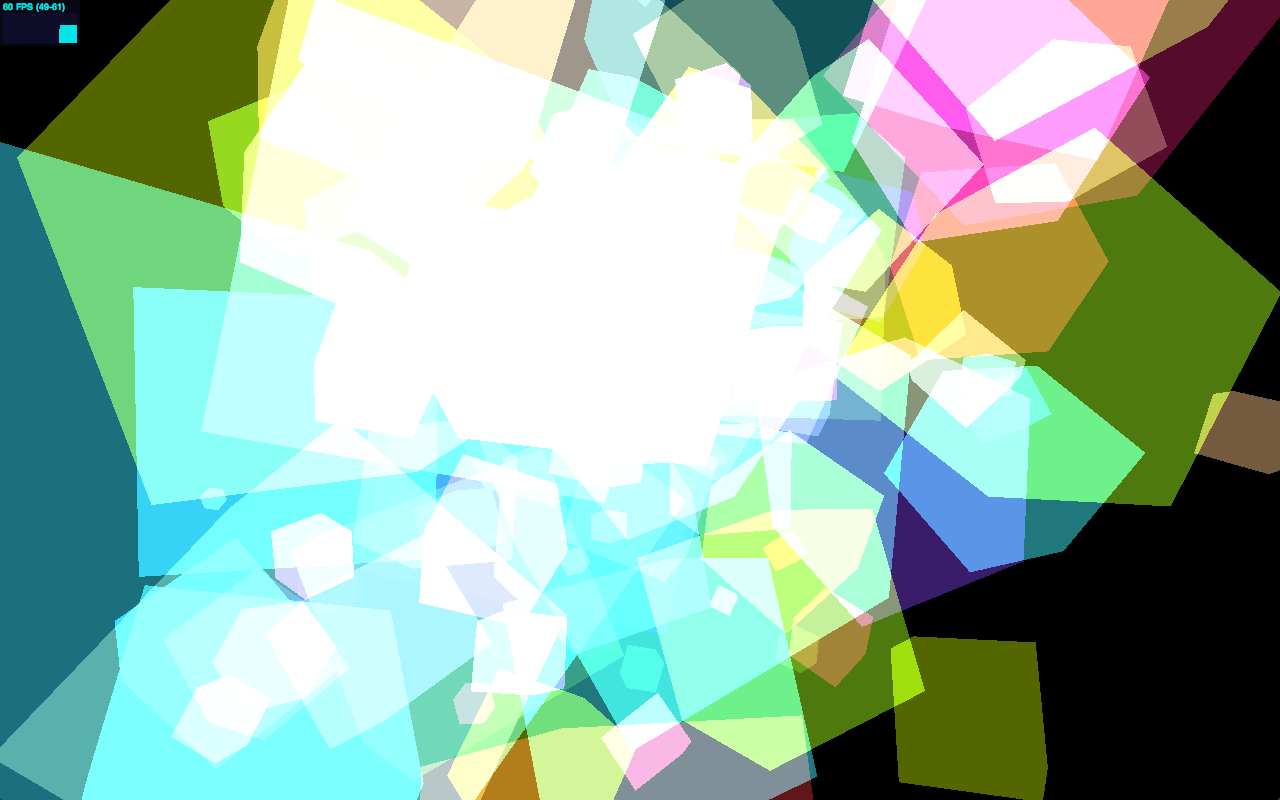
\includegraphics[height=\imgheight,width=\imgwidth]{webgl-javascript-60fps}
	\footnotesize\hspace{8\baselineskip}
	Figura 11: Demo com mais de 100 cubos semi-transparentes
	também sendo executado com WebGL e Javascript a 60 fps \\
	Fonte: \cite{website:webglperformance}
  \label{img:webgl-javascript-60fps}
\end{figure}

O estado dos navegadores na data de escrita desse
trabalho suporta a execução de jogos casuais simples, que exigem
um processamento aceitável do dispositivo, ou seja, jogos em duas
dimensões, com cálculos de física básica. O jogo pode ser otimizado
para evitar gasto desnecessário de processamento, e menor utilização
de memória, com isso há uma grande possibilidade de que o mesmo
funcione sem grandes problemas e com uma performance aceitável em dispositivos
que possuem menor poder de processamento, como os celulares por exemplo.
Alguns computadores já possuem suporte para tecnologias como WebGL e
vários navegadores como Chrome, Firefox, Safari e novas versões do
Opera, já possuem uma implementação do mesmo, mas a performance ainda
varia dependendo do suporte dos \textit{drivers} e do navegador em
questão.

\subsection{Portabilidade}

Sempre que um jogo casual é desenvolvido, tem-se em mente que ele deve
abranger a maior quantidade de dispositivos possível, para assim
atingir um maior publico, e ser utilizado onde o jogador estiver (como
é o caso dos dispositivos móveis). Quando a tecnologia para o
desenvolvimento do jogo é escolhida esse quesito tem que ser
ponderado, pois ele vai ditar em qual tipo de plataforma o jogo em
questão será executado, pois dependendo da plataforma escolhida o jogo ficará preso
a um determinado fabricante ou dispositivo.

No caso de jogos desenvolvidos para a web, esse problema acontece com as
tecnologias que utilizam \textit{plugins} que devem ser instalados na
plataforma final, pois o desenvolvedor vai depender de uma empresa
terceira (nesse caso, o desenvolvedor do \textit{plugin} para essa tecnologia),
que na maioria dos casos utiliza código proprietário, impedindo que o
próprio desenvolvedor desenvolva o \textit{plugin} para essa outra plataforma,
e o jogo desenvolvido se torna dependente das plataformas em que o
\textit{plugin}
funciona.

Um grande exemplo de problema pode ser notado com o Adobe Flash, que possui
\textit{plugin} para varios navegadores e funciona muito bem em sistemas Windows,
mas tem uma qualidade não muito boa em sistemas derivados de Unix como
o Mac OS ou o Linux. Além desse baixa qualidade nos computadores, o
Flash não possui uma versão para os celulares da Apple, assim tirando
do desenvolvedor que escolher essa plataforma uma valiosa quantia de
jogadores que poderiam pagar pelo produto. O Flash possui uma versão
para celulares com o sistema operacional Android, mas a qualidade
também não é muito boa não trazendo muito sucesso para a plataforma em
dispositivos móveis.


No caso de jogos feitos com HTML5 e Javascript, a única dependência é
o navegador, que todos os dispositivos que acessam a internet possuem,
e assim como \citeonline{davison2005killer} mostra em seu livro com
Java, tudo depende da plataforma em que uma determinada aplicação está
sendo executada, no caso do Java o jogo vai ter mais performance ou
mais recursos dependendo da implementação do Java para aquela
plataforma. O mesmo acontece com os navegadores, o jogo vai possuir
uma melhor performance ou mais funcionalidades dependendo da plataforma que
o navegador está sendo executado. Grande parte dos dispositivos que
possuem um poder de processamento considerável também possuem suporte
as novas funcionalidades do HTML5, criando a mistura adequada para a
execução de jogos casuais.

Alguns dispositivos que atualmente possuem um navegador com suporte às
funcionalidades que o HTML5 especifica são celulares com o sistema
operacional Android e celulares da Apple com sistema operacional iOS,
também desenvolvido pela Apple.
Ambos os celulares possuem um navegador capaz de rodar jogos feitos
com Canvas com uma performance razoável dependendo do hardware do
aparelho. No caso de computadores de mesa e notebooks, os navegadores
podem ser instalados gratuitamente e muitas vezes apenas a atualização
do navegador que vem por padrão no sistema operacional basta para que
um jogo seja executado sem maiores problemas.

\subsection{Fragmentação}

Quando um jogo é desenvolvido para ser executado em diversas plataformas
(conhecidos como jogos multiplataforma) é muito provável que o
desenvolvedor terá que lidar com um problema de fragmentação, pois
para cada tipo de dispositivo o jogo terá que ser customizado de uma
maneira diferente dependendo da tecnologia que foi escolhida para o
desenvolvimento do mesmo.

Os desenvolvedores que usam as tecnologias que dependem de \textit{plugins} para executar o
jogo não sofrem muito com a fragmentação, pois o \textit{plugin} gerencia
grande parte das diferenças entre os dispositivos, permitindo ao
desenvolvedor se preocupar apenas com a lógica do jogo. Dependendo do
\textit{plugin} utilizado, alguns poucos problemas podem chegar ao
desenvolvedor, como o tamanho de tela, por exemplo, pois ao jogar em
um dispositivo com uma tela menor (um celular, por exemplo), o jogo
deve se adaptar ao novo formato, e dependendo das características do jogo, o
programador terá que lidar com as diferenças e adaptar o jogo aos
vários tamanhos de tela.

Ao utilizar HTML5 o navegador se torna a plataforma de execução do
jogo, portanto ele funcionará em todos os dispositivos que
suportarem o mesmo, com a vantagem de já estar instalado previamente
no dispositivo em questão.
Independente do navegador já estar instalado no sistema, o
desenvolvedor do jogo terá os mesmos problemas dos \textit{plugins}, ou seja,
também terá de lidar com as diferenças no tamanhos das telas dos
dispositivos móveis.

A comunidade de desenvolvimento vem se preparando para esse problema e
já começam a ser discutidas possíveis soluções para esse problema.
Conforme \citeonline{html5screensize}, uma das possíveis soluções seria a
utilização do sistema MVC (modelo, visualização e controlador), onde é
possível separar a apresentação do conteúdo em várias fases, asssim
tratando a fase de visualização de forma diferente dependendo do tipo
de dispositivo em que a aplicação for executada.

Uma das desvantagens do HTML5 sobre as outras tecnologias é a versão
dos navegadores que pode ser diferente em cada dispositivo, assim
aumentando o problema de fragmentação. Esse problema é conhecido pelos
desenvolvedores web, e não é um grande problema quando definido um
requisito mínimo para se utilizar determinada aplicação. Um exemplo
simples desse problema é o jogo demo Quake III, que por ter seu código
aberto está sendo portado para rodar com WebGL diretamente no navegador.
\cite{website:webglquake3}. Quando esse jogo é acessado por um
dispositivo que não possui suporte a WebGL o jogo não irá funcionar,
pois ele depende dessa plataforma para sua execução, portanto, quando
um jogo precisa de uma determinada funcionalidade para funcionar, e
essa funcionalidade ainda não é suportada por todos os navegadores
mais conhecidos, o usuário precisa ser informado do motivo dele não
conseguir executar o jogo ao acessá-lo. O mesmo acontece com as
tecnologias que necessitam de \textit{plugins}, pois se o \textit{plugin} não estiver
instalado no dispositivo do jogador o jogo não será executado.

O escopo desse trabalho são jogos casuais, assim excluiremos jogos
maiores como é o caso do exemplo acima, portanto para a maioria dos
casos é possível ter uma segunda alternativa para que o jogo seja
executado, mesmo que para isso a performance seja inferior.

\subsection{Supote e recursos facilitadores para desenvolvimento}

Cada tecnologia disponibiliza diferentes ferramentas para facilitar o
desenvolvimento em sua plataforma, para isso algumas utilizam meios
gráficos, como ferramentas WYSIWYG que facilitam o posicionamento de
objetos e outras apenas disponibilizam suas bibliotecas como um
framework para facilitar tarefas de código.

A Adobe possui o produto Adobe Flash professional. \cite{website:adobeflash}.
Esse produto possibilita ao desenvolvedor um acesso rápido às ferramentas de cores
e desenhos, e facilita muito o posicionamento e a transição entre o
código e a amostragem do jogo, integrando os dois lados em uma única
plataforma, o que facilita o trabalho para o desenvolvedor
inexperiente.

O Unity editor é o editor da engine Unity3D que possibilita toda a
criação do jogo utilizando a plataforma, permitindo, por exemplo, a
qualquer momento clicar no botão de iniciar e testar como está a sua
criação, emulando a plataforma que você deseja publicar. \cite{website:unity3d}.
Esse editor possui a facilidade de arrastar objetos e programá-los
facilmente, o que é totalmente necessário para um jogo 3D (que e o
foco do Unity3D).

Java não possui uma ferramenta diferente para o desenvolvimento de
jogos, apenas segue o mesmo padrão de desenvolvimento convencional
Java e utiliza as bibliotecas de applet para preparar o jogo para
funcionar na web, ou seja, com uma das conhecidas IDEs (Eclipse por
exemplo) você consegue desenvolver um jogo casual em Java.

O HTML5 ainda não possui muitos recursos gráficos para facilitar no
desenvolvimento de jogos, mas muito já está sendo desenvolvido. Um dos
exemplos disso é a própria Adobe (criadora do Flash), que está
desenvolvendo uma ferramenta parecida com o Flash, que irá gerar
HTML5, Javascript e CSS para fazer animações, essa ferramenta é o
Adobe Edge, que já tem um preview disponível
gratuitamente para os desenvolvedores. \cite{website:adobeedge}.

Outras empresas também estão trabalhando para oferecer engines para
desenvolvimento de jogos para o navegador, como é o caso da Rocket
Pack \cite{website:rocketpack}, que está desenvolvendo a Rocket Engine,
que ainda não suporta Canvas, mas já
exporta HTML5 utilizando elementos DOM para diagramar o conteúdo do
jogo no navegador. \cite{website:rocketengine}.

Há empresas desenvolvendo ferramentas pagas que ajudam no
desenvolvimento de um jogo em HTML5. Uma dessas ferramentas, ou
frameworks, é a \citeonline{website:impactjs}. Esse \textit{framework}
provê um conjunto de ferramentas e utilitários para facilitar a
criação de um jogo, incluindo ferramentas para avaliar a performance,
construtores de níveis para jogos 2D, versão para celulares,
integração com engines que simulam física e outras coisas que
realmente facilitam a tarefa de desenvolver um jogo casual.

Além das ferramentas e comunidades, como é comum entre as tecnologias
mencionadas nesse trabalho, o HTML5 possui também algumas empresas que
apoiam e contribuem para seu crescimento. Um exemplo de empresa que
está apoiando com material é o Facebook, que possui uma página
dedicada aos desenvolvedores que pretendem criar aplicativos ou jogos
utilizando HTML5 para a rede social. \cite{website:facebookhtml5}.

Outras grandes empresas publicam materiais ou estão por trás do
desenvolvimento do HTML5, como é o cado da Google e da Apple. A Google
possui vários meios para divulgar informações sobre o HTML5, o mais
famoso deles é provavelmente o \citeonline{website:html5rocks} que
sempre divulga novidades sobre o que pode ser feito com as novas
tecnologias da especificação. Além dos meios de comunicação de
conteúdo, tanto a Google como a Apple contribuem com o desenvolvimento
da especificação do HTML5, como é possível ver em
\citeonline{website:w3cgoogle} e \citeonline{website:w3capple} na
seção de editores.

\subsection{Jogos criados}

O Adobe Flash possui a maior quantidade de jogos desenvolvidos para a
internet, sendo que os jogos mais conhecidos pelos usuários da
internet são feitos com o Adobe Flash. Um exemplo de jogo feito com
essa tecnologia é o Farmville. \cite{website:farmville}. Ele é um jogo
feito para a rede social Facebook, sendo ele um dos jogos mais
conhecidos da rede social e  possui uma grande quantidade de
jogadores espalhados pelo mundo.

Os applets Java foram bastante utilizados no início do desenvolvimento
de jogos para a internet, mas perderam
bastante espaço depois do surgimento do Adobe Flash e atualmente
são bem pouco utilizados para o desenvolvimento de
jogos, sendo mais utilizado para trabalhos acadêmicos.
Como os applets Java tiveram maior sucesso antes da época das redes
sociais, a maioria dos seus jogos são simples e apenas para um
jogador. Um exemplo desse tipo de jogo é o 3D-BOX,
que é um jogo simples de ação e lógica. \cite{website:3dbox}.
Outros jogos desenvolvidos com applets Java e que seguem o mesmo estilo do 3D-BOX
podem ser encontrados no site Freeware Java. \cite{website:freewarejava}.

O Unity é uma tecnologia nova mas está ficando cada vez mais popular e alguns de seus jogos
possuem versão para a web, como é o caso do jogo Battlestar Galactica
Online. \cite{website:unitybattlestargalactica}. Esse jogo reflete a
história da série Battlestar Galactica e possui uma grande quantidade
de jogadores que podem utilizar a rede social Facebook para desafiar
os amigos, o que ajuda a trazer cada vez mais jogadores.
Uma lista de jogos desenvolvidos para a web com Unity pode ser visto
no site oficial da \textit{engine}. \cite{website:unity3dwebgames}.

O HTML5 está a pouco tempo na área de desenvolvimento de jogos, mas já
possui alguns jogos interessantes, um exemplo é o jogo
WarAnimals. \cite{website:waranimals}. Esse jogo foi criado para a rede social
Facebook e já possui uma boa quantidade de jogadores. Alguns outros
jogos simples que já foram mencionados anteriormente estão ganhando versões em HTML5
como é o caso do \citeonline{website:angrybirds} e do
\citeonline{website:emberwind}.
